% 
\chapter{Estado da Arte} % Main chapter title
\label{chap:EA} % For referencing the chapter elsewhere, use Chapter~\ref{EA}

Para uma solução mais eficiente e prática, surgiu uma necessidade no ambiente empresarial que levou à pesquisa de diversas tecnologias.

No contexto em que o problema está descrito, é importante procurar aplicações e soluções desenvolvidas por outras empresas e verificar as funcionalidades básicas que estas disponibilizam aos utilizadores.

Neste capítulo, o leitor irá observar as principais funcionalidades que outras aplicações disponibilizam e de que forma contribuíram para o desenvolvimento da solução.

%-------------------------------------------------------------------------------

\section{Trabalhos relacionados} 
\label{sec:TR} 

Nesta secção estão apresentadas 5 empresas que têm como uma \textit{features} da sua aplicação o \textit{streaming}. Servirá para identificar funcionalidades que auxiliaram o projeto, bem como as funcionalidades discutas com a empresa.

Ao longo dos subcapítulos, vão ser explicados os diferentes protocolos de transmissão em direto, usados pelas diferentes empresas, que após discussão com a equipa foram escolhidos com base na sua latência e na sua complexidade.

\subsection{Youtube}

\textit{YouTube Live} tem diversas \gls{API} oficiais em Java, Python, Node.js, Go, Ruby e PHP, usadas para automatizar a programação de \textit{lives}, \textit{chat}, e metadados. A ingestão de vídeo suporta \gls{RTMP} e também \gls{HLS} para \textit{push} a partir de \textit{encoders} compatíveis. O reprodução ao utilizador é feita sobre HLS, com diversos tipos de latência.\cite{YouTube_Client_Live_Streaming_API}

Entre as principais funcionalidades desta plataforma encontrou-se:

\begin{itemize}
    \item Métricas em tempo real como: perdas de \textit{frames}, \textit{bitrate}, alertas de estabilidade.
    \item Pausa e retorno durante a transmissão.
    \item Moderação do chat
    \item Legendas automáticas e em tempo real
\end{itemize}

A interface gráfica da é intuitiva, responsiva e moderna. Permite, assim, ao
criador uma navegação eficiente e acessível pelas funcionalidades da aplicação.

\begin{figure}[H]
\centering
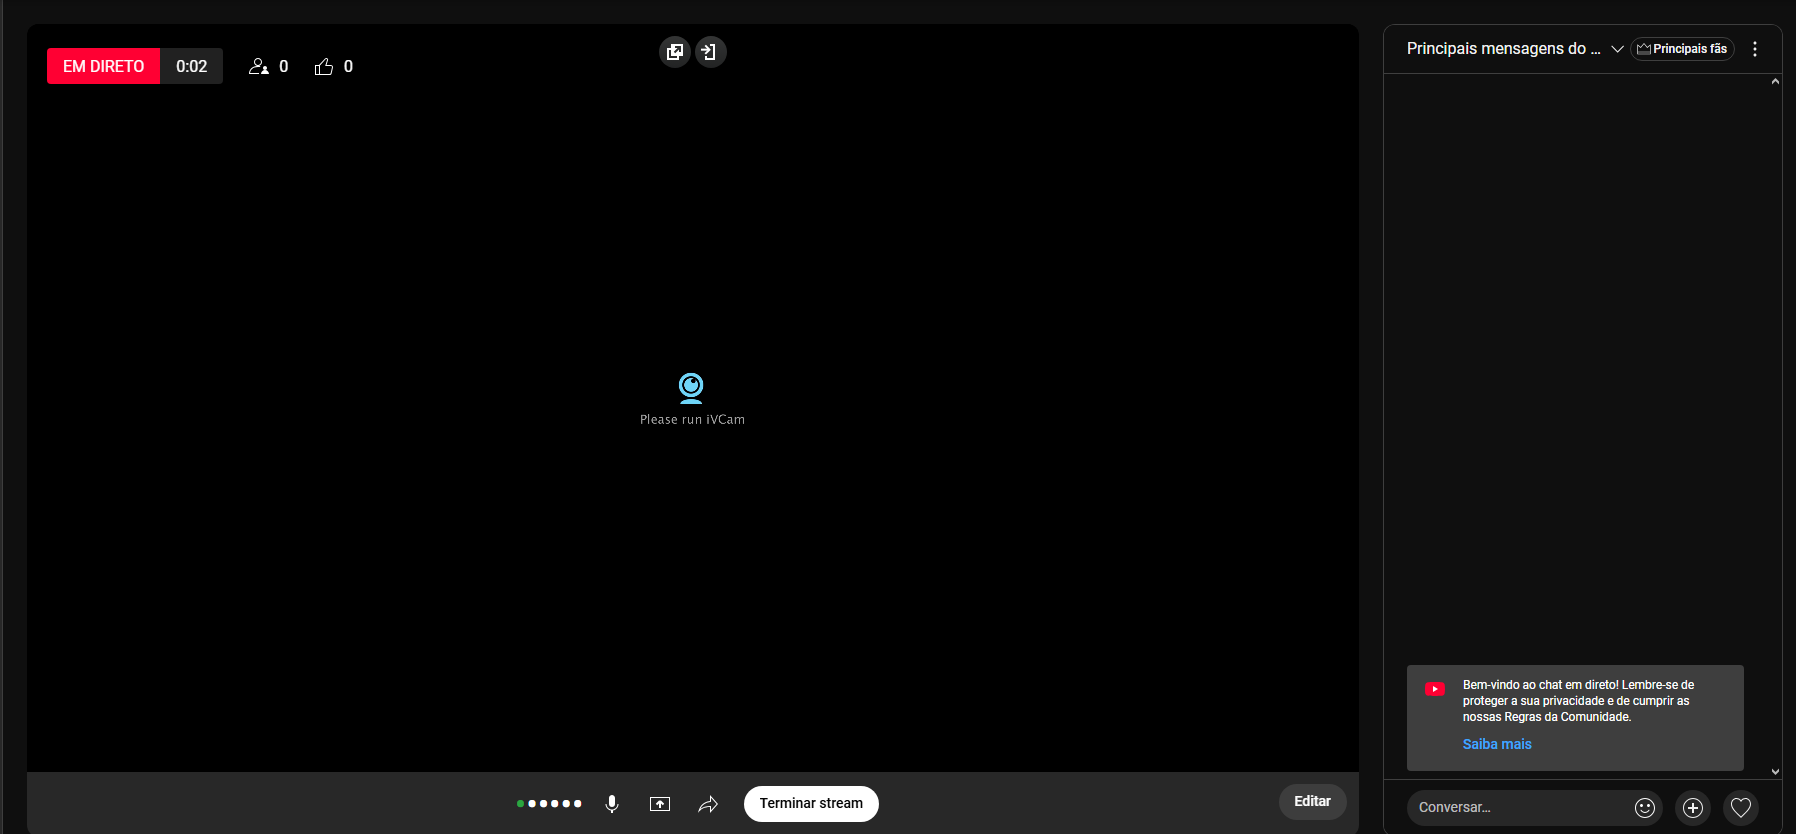
\includegraphics[width=1\textwidth]{frontmatter/assets/yt3.png}
\caption{Interface de Criador de Conteúdo do Youtube Live \cite{Youtube}}
\label{fig}
\end{figure}

A escolha do microfone, câmara, titulo e descrição são efetuadas nas etapas antes de iniciar a transmissão. Para além destas etapas a plataforma permite a mudança destas funcionalidades durante a transmissão. 

A \textit{livestream} pode ser efetuada em diversos dispositivos, com etapas semelhantes, e com diferentes programas que facilitam a transmissão de conteúdo. 

\paragraph{Pontos Fortes}
\begin{itemize}
  \item Alcance e robustez de infraestrutura.
  \item Transcodificação automática para múltiplas qualidades (\textit{bitrate}).
  \item Ferramentas nativas de monetização (anúncios, \textit{Super Chat}/\textit{Stickers}, \textit{Memberships}).
  \item Analítica integrada em tempo real.
\end{itemize}

\paragraph{Pontos fracos}
\begin{itemize}
  \item Navegação inicial mais longa, com um excesso de menus para o criador.
  \item Inserção de anúncios pode interromper o ritmo do \textit{chat} se usada sem planeamento.
  \item Títulos, restrições e visibilidades exigem \textit{checklist} para evitar deslizes.
  \item Difícil expansão dentro da plataforma.
\end{itemize}


\subsection{KICK}

As integrações disponibilizadas pela \textbf{Kick} assentam numa API pública REST/JSON, com endpoints para canais, utilizadores, \textit{chat}, moderação e \textit{livestreams}. O \textit{ingest} de vídeo para criadores é realizado por RTMP/RTMPS configuradas num \textit{encoder} (ex: OBS).

A plataforma disponibiliza as principais funcionalidades:

\begin{itemize}
    \item Creator Dashboard.
    \item \textit{Replays} automáticos após terminar a transmissão.
    \item Monetização mais abrangente.
    \item \textit{Co-stream} nativa.
\end{itemize}

Numa perspetiva de visualizador, a plataforma apresenta uma interface focada especialmente no vídeo. A interação com a comunidade é feita via \textit{low latency chat}, com emojis e difetentes cores para cada utilizador.

\begin{figure}[H]
\centering
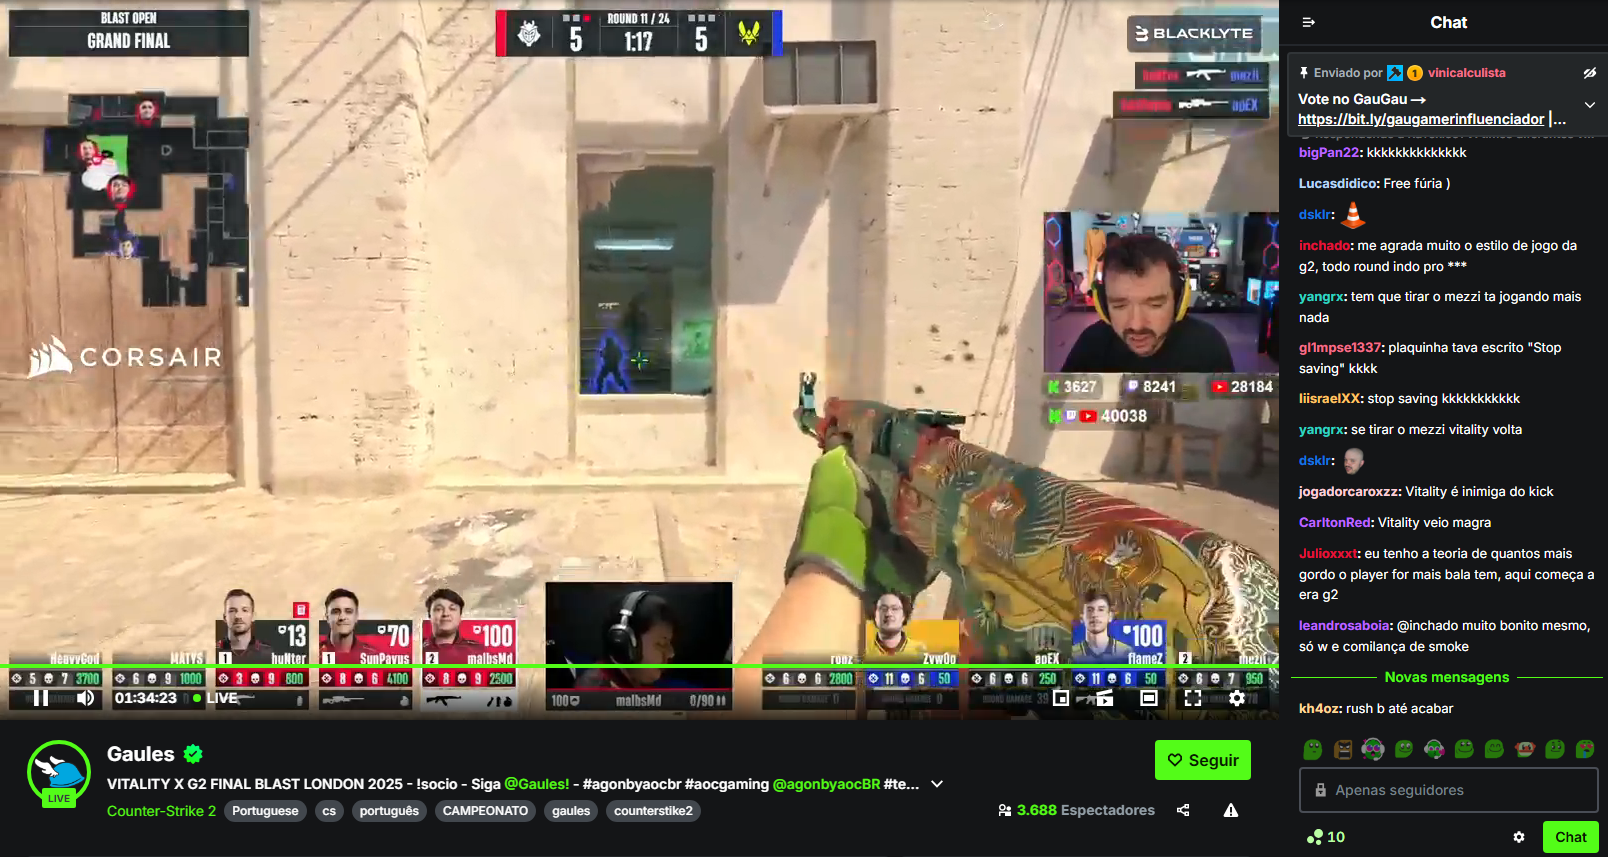
\includegraphics[width=1\textwidth]{frontmatter/assets/kick.png}
\caption{Interface de utilizador da Kick \cite{KickGaulesChannel}}
\label{fig}
\end{figure}

A configuração de utilizador é pouca o que permite assistir a uma transmissão ao vivo rapidamente, além disso, o utilizador tem diversas maneiras de interagir com o criador, podendo tirar excertos da \textit{stream}, paritcipar em sondagens, doar, e mandar mensagem privada ao mesmo.

\paragraph{Pontos fortes}
\begin{itemize}
  \item Fluxo de arranque simples.
  \item Ferramentas de moderação claras.
  \item Condições de monetização competitivas.
\end{itemize}

\paragraph{Pontos fracos}
\begin{itemize}
  \item Ecossistema de extensões e API ainda em evolução.
  \item Dependência de serviços externos.
  \item Documentação pública de protocolos de entrega pouco detalhada.
\end{itemize}

\subsection{Twitch}

A \textbf{Twitch Live} foi apresentado pela \textbf{Twitch Interactive} em 2011, após a aquisição pela \textbf{Amazon} em 2014\cite{Twitch2011LaunchAmazon2014}. A \textbf{Twitch} expõe uma \textbf{API REST}, \textit{webhooks} e \textit{EventSub} via \textit{WebSocket}. O principal ecossistema usa \textit{JavaScript}/\textit{TypeScript} para o chat e \textit{Java}/\textit{Kotlin}, C\#, Python e Go para as restantes API's. Durante a transmissão o \textit{ingest} é feito por RTMP a entrega ao público é por HLS.

As principais características da plataforma de \textit{streaming} são:

\begin{itemize}
    \item Painéis personalizáveis para o estado do stream, \textit{chat}, alertas, \textit{stream markers}...
    \item Baixa latência.
    \item Co-stream nativo
    \item Monetização integrada.
    \item Extensões personalizáveis para melhorar a analítica da transmissão.
\end{itemize}

A interface embora interativa e personalizável, dispões de uma poluição visual grande, existem imensas definições e características que numa primeira interação podem desmotivar o criador a iniciar a transmissão.

\begin{figure}[H]
\centering
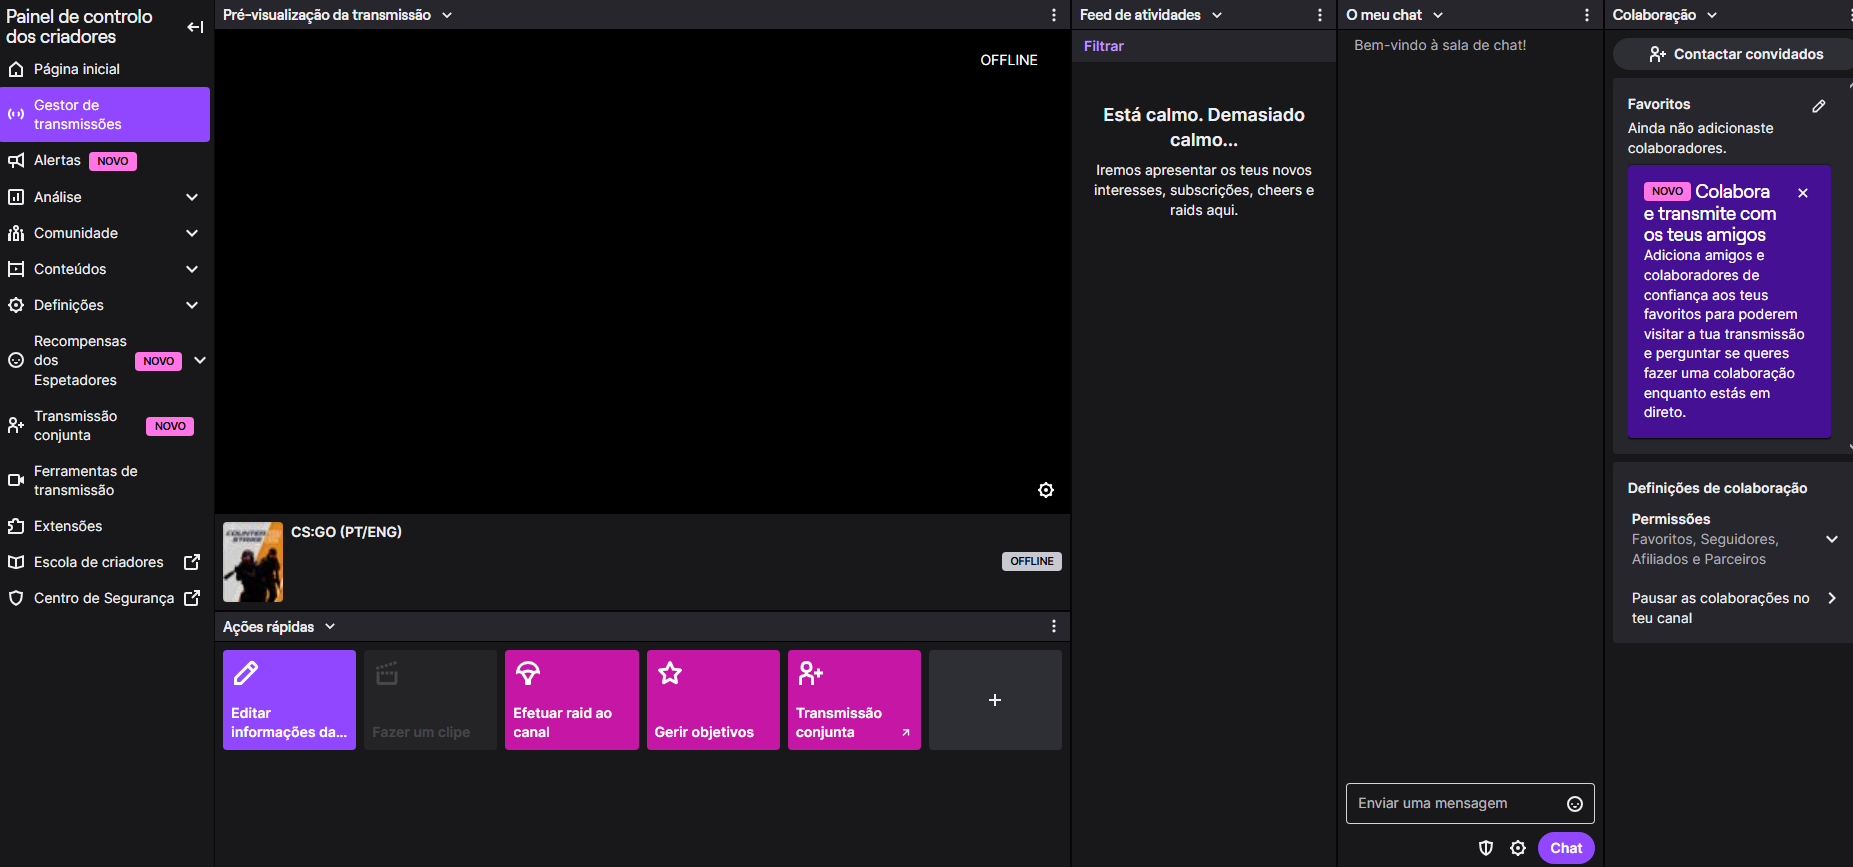
\includegraphics[width=1\textwidth]{frontmatter/assets/twitchcriador.png}
\caption{Interface de Criador de Conteúdo da Twitch \cite{Twitch}}
\label{fig}
\end{figure}

Contudo, a disposição de menus e opções descritivas ajudam o criador mais técnico a personalizar o seu ambiente e a uma melhor interação com a sua comunidade.


\paragraph{Pontos fortes}
\begin{itemize}
  \item Painel de transmissão personalizável
  \item Grande número de ferramentas de moderação.
  \item As extensões permitem uma grande personalização do ecossistema.
  \item Padrões de interação rápida como por exemplo: chat, \textit{emojis} e criação de excertos da transmissão pelos utilizadores.
\end{itemize}

\paragraph{Pontos fracos}
\begin{itemize}
  \item \textit{Dashboard} denso.
  \item Monetização com regras restritas.
  \item Gestão de anúncios sensível, pois podem colidir com momentos importantes do conteúdo.
  \item Contínua mudança de nomenclatura das definições.
\end{itemize}


\subsection{TikTok}

O TikTok disponibiliza diferentes SDK's para Android, IOS e Web, existem ainda \textit{Webhooks} e \textit{APIs} para integrações do lado do servidor.

Para o \textit{streaming}, o \textit{ingest} do ambiente é feito por RTMP/RTMPS ou por algum \textit{encoder} externo. A entrega aos utilizadores é feita por HLS.

\begin{figure}[H]
\centering
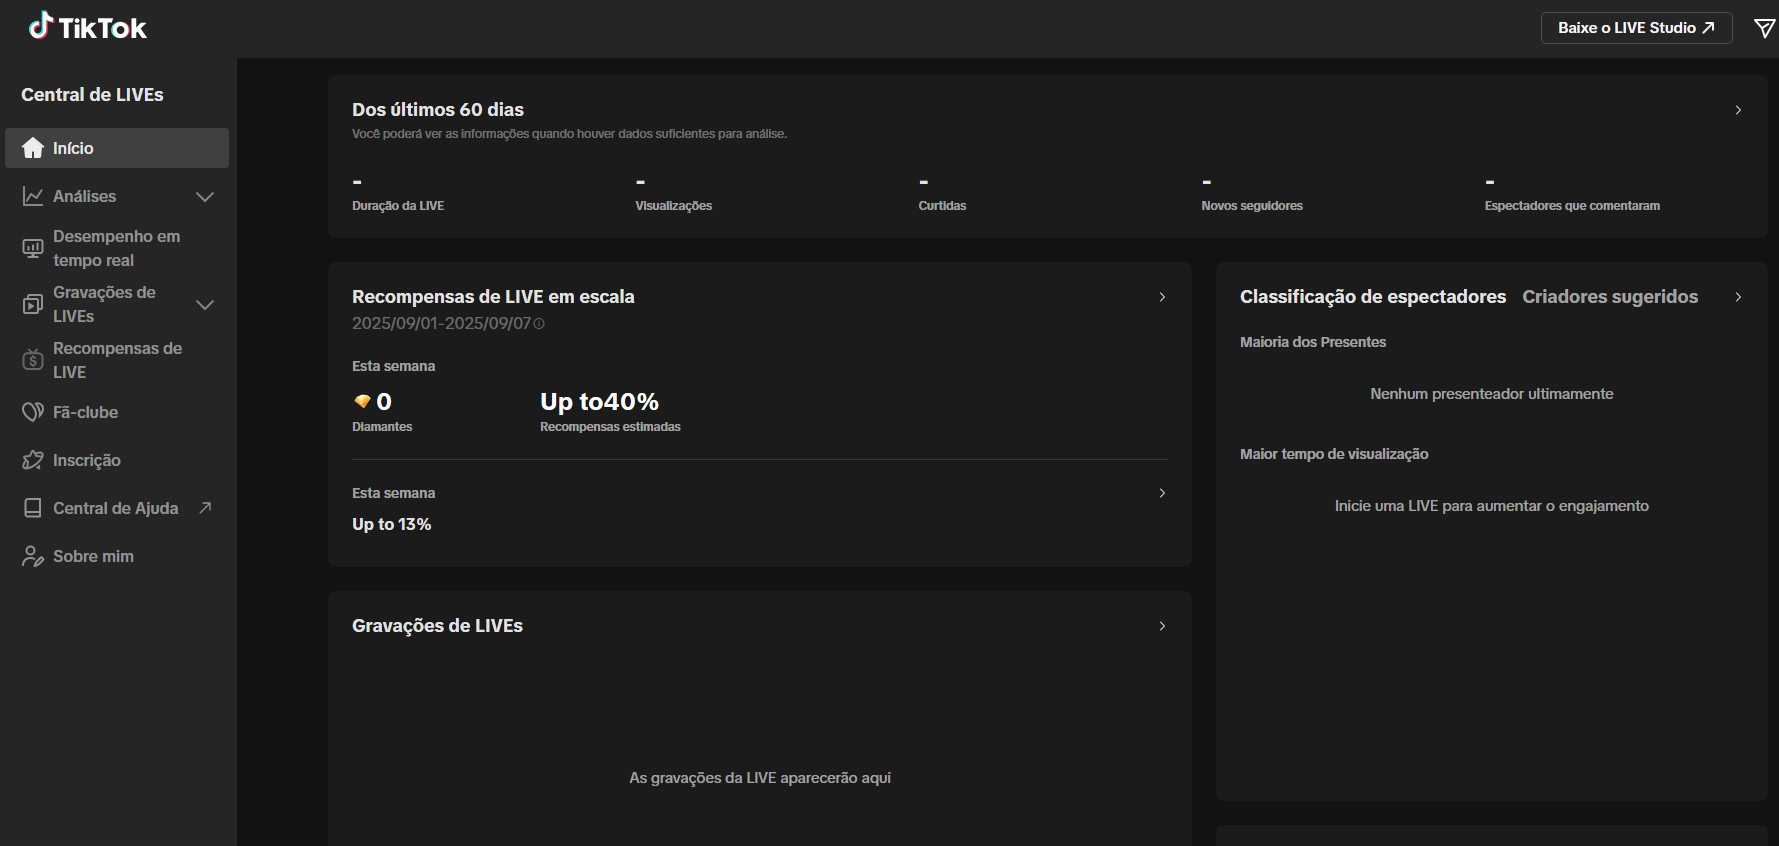
\includegraphics[width=1\textwidth]{frontmatter/assets/tiktok.png}
\caption{\textit{LIVE} center do \textbf{TikTok}}
\label{fig}
\end{figure}

Organizado em barra lateral, cabeçalho e grelha de cartões informativos, a interface mostra uma \textit{dashboard} necessária para uma expansão na aplicação, pois todas as transmissões são personalizáveis em termos de interação e moderação.

O controlo da \textit{livestream} está totalmente dependente do utilizador, mas por outro lado todos os dados da transmissão são disponibilizados ao criador, com foco na monetização e transações com uma moeda interna.


\paragraph{Pontos fortes}
\begin{itemize}
  \item Monetização nativa.
  \item Presentes e efeitos destacam-se e mantêm o público a participar.
  \item \textit{Co-stream} predefinidos e convites em poucos passos.
\end{itemize}

\paragraph{Pontos fracos}
\begin{itemize}
  \item Ambiente visual poluído.
  \item Limita criadores que trabalham noutros sistemas, pois o encoder internos funciona apenas no \textit{Windows}.
  \item Prioridade ao formato vertical.
\end{itemize}


\subsection{Discord}

O \textbf{Discord Go Live} foi apresentado pela \textbf{Discord Inc.} em 2019. O seu desenvolvimento foi feito sobretudo em \textit{JavaScript}/\textit{TypeScript}, \textit{Python}, \textit{Go} e \textit{Java}. Possui sobretudo \textit{API's REST} e \textit{WebSocket's} oficiais. Para voz e vídeo, as ligações usam \gls{RTP}/\gls{UDP}. Diferente de plataformas anteriormente referidas o \textit{broadcast} não é nativo no cliente, mas sim com retransmissão pelo \textit{backend}.

\begin{figure}[H]
\centering
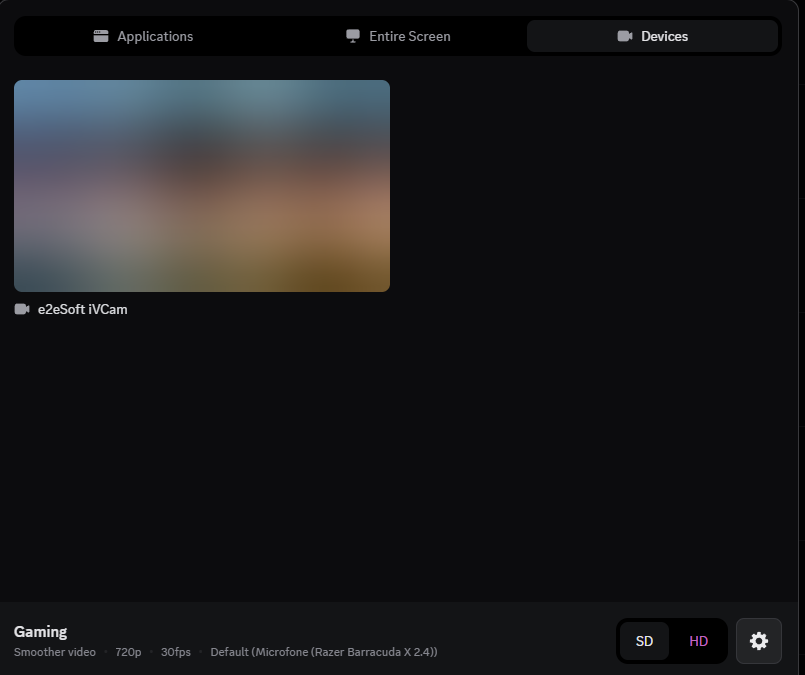
\includegraphics[width=1\textwidth]{frontmatter/assets/discord.png}
\caption{Escolha de cenário para transmissão}
\label{fig}
\end{figure}

A interface foca-se na seleção de fonte para a transmissão com três zonas principais.

A barra de separadores, contêm diferentes de secções, em que o utilizador pode escolher entre partilhar alguma aplicação especifica, partilhar o ecrã inteiro ou escolher algum dispositivo para iniciar a transmissão.

O rodapé mostra algumas definições de controlo como o tema, a qualidade e o dispositivo de áudio. Este controlo dado pela plataforma mostra que nao é necessario alguma configuração por parte do utilizador para definidir tanto os dispositivos de entrada como os de saída.

\paragraph{Pontos fortes}
\begin{itemize}
  \item Partilha de ecrã sem assistentes longos.
  \item Vídeo, voz e \textit{chat} lado a lado.
  \item Partilha de vídeo privada.
\end{itemize}

\paragraph{Pontos fracos}
\begin{itemize}
    \item Como a transmissão é só feita em "chamada" não existe crescimento na plataforma.
    \item A qualidade depende muito de transações internas
    \item Alguma partilha de conteúdo é bloqueada. 
\end{itemize}

\subsection{Tabela Comparativa das Plataformas}

Para uma melhor visualização das diferentes características das aplicações construiu-se a seguinte tabela: 

\begin{table}[H]
\caption{Tabela Comparativa das Plataformas}
\label{tab:comparacao-plataformas}
\begin{center}
\begin{tabular}{|p{5.5cm}|c|c|c|c|c|}
\hline
\textbf{Funcionalidade / Característica} &
\textbf{YouTube} &
\textbf{Kick} &
\textbf{Twitch} &
\textbf{TikTok} &
\textbf{Discord} \\
\hline
Início de transmissão intuitivo                           &   & x &   & x & x \\
\hline
Utilização de programas externo para a transmissão        & x & x & x & x &   \\
\hline
Moderação de \textit{chat}                                & x & x & x & x & x \\
\hline
Monetização nativa em direto                              & x & x & x & x &   \\
\hline
\textit{Replay} da transmissão                            & x & x & x & x &   \\
\hline
Analítica em tempo real e pós-live                        & x & x & x & x &   \\
\hline
Interação em tempo quase real (boa latência)              & x & x & x & x & x \\
\hline
Painel do criador unificado (operar tudo num ecrã)        & x & x & x & x &   \\
\hline
Extensibilidade / overlays prontos na plataforma          &   &   & x &   &   \\
\hline
Experiência otimizada na \textit{vertical}                &   &   &   & x &   \\
\hline
Experiência otimizada na \textit{landscape}               & x & x & x &  & x  \\
\hline
Alcance além de seguidores                                & x & x & x & x &   \\
\hline
Adequado a comunidades privadas                           &   &   &   &   & x \\
\hline
\end{tabular}
\end{center}
\end{table}


A Tabela~\ref{tab:comparacao-plataformas} mostra três plataformas equivalentes: \textbf{YouTube}, \textbf{KICK} e \textbf{Twitch}, pois oferecem uma experiência de \textit{broadcast} completa (monetização, \textit{replays}, analítica e painéis de criador complexos). O \textbf{TikTok} privilegia rapidez e interação social nos dispositivos \textit{mobile}. O \textbf{Discord} aposta em simplicidade e colaboração em espaços privados, prescindindo de replays e monetização nativa. Em termos de moderação e \textit{chat}, as quatro plataformas de \textit{streaming} mantêm ferramentas complexas, por outro lado, o \textbf{Discord}, foca-se na conversa em tempo real dentro do próprio canal.


\section{Tecnologias existentes} 

Após análise das tecnologias utilizadas nas soluções das diversas empresas e com as discussões em grupo com a equipa foi alcançado o conhecimento base e necessário para perceber a melhor abordagem a seguir.

\subsection{Protocolos De \textit{Streaming}}

Os protocolos de \textit{streaming} estruturam o percurso do sinal entre captura, \textit{ingest}, codificação e entrega ao público, e dependendo do protocolo pode implicar a latência e compatibilidade. A Tabela~\ref{tab:streaming-protocols-comparativa} compara os protocolos mais relevantes (RTMP/RTMPS, HLS/LL-HLS, WebRTC e MediaStream) quanto a uso típico, vantagens e limitações.

\begin{table}[H]
\centering
\caption{Resumo comparativo de protocolos de \textit{streaming}}
\label{tab:streaming-protocols-comparativa}
\begingroup
\small
\setlength{\tabcolsep}{4pt}
\renewcommand{\arraystretch}{1.05}
\begin{tabular}{|p{3cm}|p{3cm}|p{4cm}|p{4cm}|}
\hline
\textbf{Protocolo} & \textbf{Uso típico} & \textbf{Pontos fortes} & \textbf{Pontos fracos} \\
\hline
RTMP/RTMPS \cite{Chang2011RTMPHTTP} & \textit{Ingest} do criador & Configuração simples e uma alta compatibilidade com diversos \textit{enconders}. & Sendo um dos primeiros protocolos tem uma latência maior. \\
\hline
HLS / LL-HLS \cite{Bentaleb2022LLDASHHLS} & Entrega ao utilizador & Tem um amplo suporte tanto em \textit{web} como em \textit{mobile}, a versão de baixa latência melhoras o desempenho do HLS clássico & O HLS clássico apresenta uma latência considerável (15-30), LL-HLS pede mais poder computacional mas entrega com pouco \textit{delay} \\
\hline
WebRTC \cite{Nurminen2013P2PWebRTC} & Interatividade e baixa latência & Um dos protocolos com a menor latência, bidirecional e nativo do \textit{browser}. & O escalonamento é condicionado pelos custos elevados. \\
\hline
{MediaStream} & Captura local no \textit{browser} & Nativo nos \textit{browsers} modernos, acesso direto a câmara e microfone. & Requer combinação com WebRTC/RTMP para \textit{ingest} e dependente de permissões do utilizador e políticas de segurança do \textit{browser}. \\
\hline
\end{tabular}
\endgroup
\end{table}



\subsection{Back-End}

% Introdução — BE
No \textit{back-end}, as decisões impactam o desempenho das APIs, a fiabilidade dos serviços e a escalabilidade de fluxos críticos (autenticação, gestão de sessões, monetização e VOD). A Tabela~\ref{tab:be-comparativa} resume as lingaguem correntes, com ênfase em modelos arquiteturais.


\begin{table}[H]
\caption{Tabela resumo das tecnologias \textit{back-end} (BE)}
\label{tab:be-comparativa}
\begin{center}
\small
\begin{tabular}{|p{2.4cm}|p{2.5cm}|p{4cm}|p{4cm}|}
\hline
\textbf{Linguagem / Framework} & \textbf{Arquitetura} & \textbf{Pontos fortes} & \textbf{Pontos fracos} \\ \hline
Node.js (Express) & REST/GraphQL, microserviços & Mesma linguagem do FE, NPM vasto, 
 produtividade alta. & \textit{CPU-bound} menos eficiente, \textit{package} com eficiencia desigual. \\ \hline
Python (FastAPI) & Comaptibilidade REST, microserviços & Desenvolvimento rápido, boa documentação, desempenho adequado. & Limita as tarefas \textit{CPU-Bound}, dependências podem crescer. \\ \hline
Java (Spring Boot) & Monólito/modular, microserviços & Robustez empresarial, ecossistema amplo & Consumo de memória e \textit{startup} maiores, curva de aprendizagem. \\ \hline
Go & Serviços leves, REST & Concorrência simples e baixo uso de recursos. & Ecossistema web menos abrangente. \\ \hline
PHP & Monolítica & Compatibilidade elevada e facil integração com o Front-End & Falta de padronização e de continuidade \\ \hline
\end{tabular}
\end{center}
\end{table}

\subsection{Front-End}

A escolha da tecnologia \textit{front-end} condiciona desempenho e experiência do utilizador, live dashboards. Na Tabela~\ref{tab:fe-comparativa} sintetizam-se as opções mais usadas, destacando arquitetura, pontos fortes e limitações práticas relevantes para produtos de vídeo em direto.

% ==============================
% Tabela — Front-end (FE)
% ==============================
\begin{table}[H]
\caption{Tabela resumo das tecnologias \textit{front-end} (FE)}
\label{tab:fe-comparativa}
\begin{center}
\small
\begin{tabular}{|p{2.4cm}|p{2.5cm}|p{4cm}|p{4cm}|}
\hline
\textbf{Linguagem / Framework} & \textbf{Arquitetura} & \textbf{Pontos fortes} & \textbf{Pontos fracos} \\ \hline

React & \gls{SPA}; \gls{SSR} via Next.js &
Responsivo, forte reutilização de componentes, comunidade ampla, boa produtividade. &
Muitas escolhas de bibliotecas, risco de inconsistências visuais, requer organização em projetos maiores. \\ \hline

Next.js (React) & SSR/ISR; \textit{routing} e \textit{data fetching} integrados &
Bom desempenho, arranque simples, páginas e rotas prontas. &
Convenções próprias, atualizações podem exigir ajustes, alguma rigidez fora do padrão. \\ \hline

Vue & SPA; SSR com Nuxt &
Aprendizagem rápida, componentes claros, documentação acessível, curva suave. &
Menor adoção corporativa, ecossistema mais reduzido, estilos de implementação podem variar entre equipas. \\ \hline

Angular & SPA; SSR com \textit{Angular Universal} &
Padrões consistentes, boas ferramentas oficiais, adequado a equipas grandes. &
Curva de aprendizagem longa, pode tornar-se pesado e menos flexível. \\ \hline

\end{tabular}
\end{center}
\end{table}

\subsection{Base de Dados}

A camada de dados sustenta contas, conteúdos, transações e métricas de audiência, exigindo combinações de armazenamento transacional e serviços orientados a desempenho. A Tabela~\ref{tab:db-comparativa} apresenta SGBD amplamente adotados, evidenciando modelos, pontos fortes e fragilidades para cenários de live/VOD.

\begin{table}[H]
\caption{SGBD e tecnologias de dados mais comuns}
\label{tab:db-comparativa}
\begin{center}
\small
\begin{tabular}{|c|c|p{3cm}|p{3cm}|}
\hline
\textbf{SGBD / Tecnologia} & \textbf{Modelo} & \textbf{Pontos fortes} & \textbf{Pontos fracos} \\ \hline
PostgreSQL & Relacional (ACID) & Muito completo e estável, extensível, bom suporte a dados modernos. & Exige afinação em projetos grandes, escala horizontal mais trabalhosa. \\ \hline
MySQL/MariaDB & Relacional (ACID) & Simples de gerir, rápido em leituras, comunidade ampla. & Menos recursos avançados, pode exigir soluções de contorno em cenários complexos. \\ \hline
MongoDB & Documento (NoSQL) & Esquema flexível, evolução rápida, adequado a dados heterogéneos. & Consistência e consultas complexas requerem desenho cuidadoso. \\ \hline
Redis & Chave–valor / \textit{cache} & Muito rápido, excelente para \textit{cache}, sessões e filas. & Persistência limitada, gestão de memória crítica, não substitui a base principal. \\ \hline
\end{tabular}
\end{center}
\end{table}

\section{Análise e seleção das tecnologias}
\label{sec:Req} 
Após análise das tecnologias utilizadas nas plataformas e com as \textit{daily meetings} com a equipa, alcançou-se o conhecimento necessário para perceber a melhor abordagem a seguir.

\subsection{Protocolos de Streaming}

Num enquadramento geral, opta-se pela captura nativa no navegador, \textit{ingest} em baixa latência com WebRTC através do \gls{IVS} Web Broadcast SDK da AWS e distribuição por HLS/LL-HLS para maximizar compatibilidade. A escalabilidade tira partido da infraestrutura  global da AWS IVS (\textit{ingest points}, transcodificação e \textit{playback}).

Para a captura, o MediaStream, suportado nativamente nos \textit{browsers} modernos permite o acesso controlado a câmara/microfone. Tal reduz complexidade ao cliente e mantém a privacidade por defeito.

Utilizou-se WebRTC via IVS Web Broadcast SDK para atingir latências muito baixas na ordem de um a três segundos. A escolha evita a manutenção de servidores próprios, delegando essa preocupação com os serviços da AWS. A presença de streamKey e ingestEndpoint garante isolamento por canal.

A reprodução é servida em HLS (com LL-HLS ativado no player via hls.js), o que assegura uma compatibilidade ampla tanto em \textit{web} como em \textit{mobile}. O IVS trata da codificação e expõe um \textit{playbackUrl}. Esta decisão equilibra latência reduzida com robustez, tolerância a variações de rede e escala global.

\subsection{Back-end}

Após a pesquisa ponderada, a equipa decidiu escolher como tecnologia principal o \textbf{Node.js} com \textit{Express}, a linguagem principal é o JavaScript, o que torna quaisquer operações \gls{I/O} rápidas e leves. Para uma plataforma de \textbf{social media} é necessário existir uma ligação com os casos de uso e com a tecnologia escolhida, para tal sabemos que um dos objetivos principais é a baixa latência e a transmissão em tempo real, logo o Node.js foi a tecnologia que a equipa se inclinou desde inicio.

Para além disso, o \textbf{Express} fornece um \textit{framework} minimalista, com \textit{routing} e \textit{middleware} (autenticação, \textit{rate limiting}, CORS), o que acelera a implementação de \textit{APIs} estáveis e testáveis.

A pilha \textbf{JavaScript} facilita a integração com SDKs AWS e suporta adoção progressiva de \textbf{TypeScript} para maior segurança estática.

\subsection{Front-end}

Para o desenvolvimento do front-end, existia uma indecisão em relação a duas
tecnologias, uma delas nunca trabalhada pela equipa e outra com conhecimento prévio pela mesma.

\begin{itemize}
    \item Biblioteca \textbf{React} do \textbf{JavaScript}
    \item Framework \textbf{Angular}
\end{itemize}

A Tabela~\ref{tab:ang-rea-comp} ajuda a comparar as duas abordagens

\begin{table}[H]
\caption{Comparação entre React e Angular}
\label{tab:ang-rea-comp}
\begin{center}
\small
\begin{tabular}{|c|c|c|}
\hline
\textbf{Funcionalidade/ Critério} & \textbf{React} & \textbf{Angular}\\ \hline
Linguagem Base & JavaScript com HTLM & TypeScript \\ \hline
Casos de uso &  SPA, Modularização, \textit{dashboards} & Grande Aplicações estruturadas \\ \hline
Curva de aprendizagem & Elevada & Moderada e flexível \\ \hline
Tipo & Biblioteca de JavaScript & Framework completo \\ \hline
\end{tabular}
\end{center}
\end{table}

A equipa decidiu escolher o \textbf{React} porque, ao combinar React, Router e JSX no cliente com Node.js/Express no servidor, resulta uma arquitetura coesa e preparada para ambientes em tempo real.

\subsection{Base de dados}

A equipa optou por SQL (Aurora PostgreSQL) para dados sensíveis, críticos e com forte exigência de integridade e segurança como: ids, \textit{usernames}, emails .... E por NoSQL (DynamoDB) para dados altamente editáveis e de apresentação como: preço, título, descrição, flags e preferências. Esta divisão maximiza coerência transacional onde é necessária e flexibilidade onde é benéfica.

\section{Conclusão}

Conclui-se que o ecossistema de \textit{livestreaming} organiza-se em três partes: transmissão pública (YouTube, Twitch, TikTok/Kick), \textit{mobile} (TikTok) e colaboração privada (Discord). A decisão deve privilegiar usabilidade do painel do criador, monetização e reaproveitamento (VOD/clips).

Em termos técnicos, prevalece RTMP para ingest, HLS/LL-HLS para entrega e WebRTC quando a latência sub-segundo é crítica. No stack, FE modernos (React/Next, Vue, Angular) e BE leves (Node.js+Express) oferecem rapidez e manutenção aceitável. 

Para dados, PostgreSQL e MySQL servem o núcleo transacional, com MongoDB/Redis a complementar flexibilidade e desempenho.


\vspace{20mm} 




